\documentclass[xcolor=pdftex,dvipsnames,table,mathserif,aspectratio=169]{beamer}
\usetheme{metropolis}
%\usetheme{Darmstadt}
%\usepackage{times}
%\usefonttheme{structurebold}

\usepackage[english]{babel}
%\usepackage[table]{xcolor}
\usepackage{pgf,pgfarrows,pgfnodes,pgfautomata,pgfheaps}
\usepackage{amsmath,amssymb,setspace}
\usepackage[latin1]{inputenc}
\usepackage[T1]{fontenc}
\usepackage{relsize}
\usepackage[absolute,overlay]{textpos} 
\newenvironment{reference}[2]{% 
  \begin{textblock*}{\textwidth}(#1,#2) 
      \footnotesize\it\bgroup\color{red!50!black}}{\egroup\end{textblock*}} 

\DeclareMathSizes{10}{10}{6}{6} 


\title [``Old'' IO]{Before there was ``New'' Empirical IO}
\author{C.Conlon}
\institute{Grad IO }
\date{Fall 2020}
\setbeamerfont{equation}{size=\tiny}
\begin{document}

\begin{frame}
\titlepage
\end{frame}

\begin{frame}{Conjectural Variations}
\small
\begin{itemize}
\item If I change my quantity, why doesn't my rival?
\item Biggest complaint about Cournot is that we hold quantities of competitors fixed
\item Suppose we did not so that $\frac{\partial Q_i}{\partial q_i} = (1 + \frac{\partial Q_{-i}}{\partial q_i}).$
\item Marginal Revenue becomes:
\begin{eqnarray*}
P + P'(Q) \cdot q_i \cdot \underbrace{\left(1+ \frac{\partial Q_{-i}}{\partial q_i} \right)}_{\theta_i}
\end{eqnarray*}
\item $\frac{\partial Q_{-i}}{\partial q_i} =-1$  or $\theta_i =0$ corresponds to competition/Bertrand (aggregate $Q$ is unchanged).
\item $\frac{\partial Q_{-i}}{\partial q_i} =0$ or $\theta_i = 1$ corresponds to the Cournot model.
\item $\frac{\partial Q_{-i}}{\partial q_i} =N-1$ or $\theta_i = N$ corresponds to the joint profit maximization
\item This was great for applied theory, now I can nest all of the classic models (PC, monopoly, Cournot) with a single parameter.
\end{itemize}
\end{frame}

\begin{frame}{Conjectural Variations: Issues}
\begin{itemize}
\item On one hand seems like more flexibility was a good thing.
\item On the other hand with some $\theta_i$ we can justify nearly anything.
\item Two questions
\begin{enumerate}
\item Can we expect to recover $\theta_i$ from data?
\item What about \alert{consistent conjectures} (ie: suppose I require firms to actually want to respond in the way that I believe they will).
\end{enumerate}
\end{itemize}
\end{frame}



\begin{frame}{Consistent Conjectures}
\begin{itemize}
\item Bresnahan (1981) posed the consistent conjectures hypothesis (one unique conjecture that satisfied all FOCs simultaneously).
\item Large theory literature that followed [see Daughety (1985) or Lind(1992)] show Cournot $\theta_i=0$ is the only consistent conjecture absent some knife-edge cases.
\item This basically meant that CV approaches fell out of favor with game theorists by the late 1980s/early 1990s.
\item Things are even more problematic for dynamic models.
\item The approach persisted in empirical work until Corts (1999) [more on this later].
\end{itemize}
\end{frame}

\begin{frame}{Can/Should we try and recover $\theta_i$ from data?}
\begin{figure}
\begin{center}
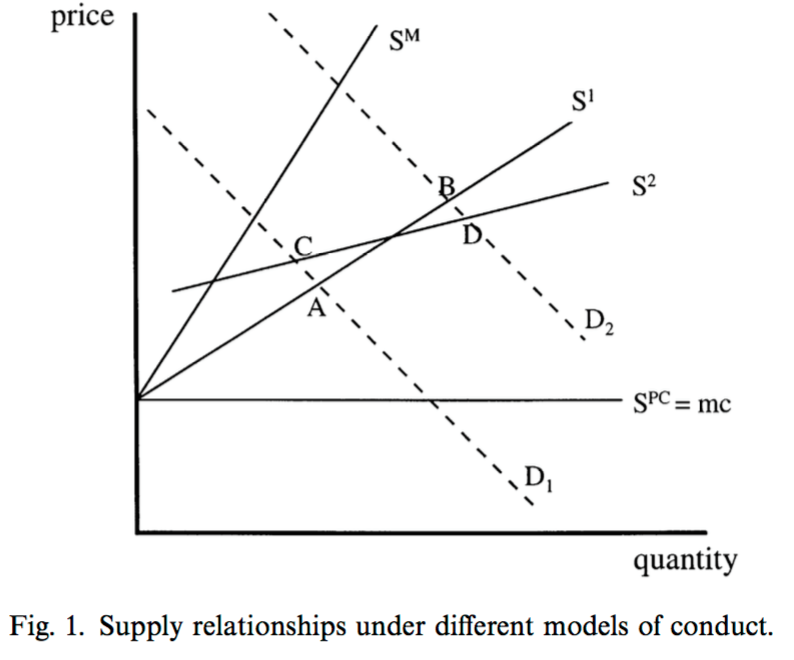
\includegraphics[width=4in]{resources/cortsfigure.png}
\end{center}
\end{figure}
\end{frame}



\begin{frame}{Testing S-C-P }
Can we test for relationship between performance and market structure?
\begin{itemize}
\item Positive correlation between $HHI$ and market power.
\begin{itemize}
\item Usually easy to measure concentration (sort of)
\item Measuring Profits is tough:
\begin{itemize}
\item Accounting profits: taxes and depreciation aren't really very close $P-MC$.
\item Tobin's Q
\item The Lerner index: $(P-MC)/P$
\end{itemize}
\item We don't usually get to observe $MC$ in data.

\begin{itemize}
\item Maybe we see something like total revenue or total variable cost and units sold.
\item Have to use unit values $(P-AVC)/P$ which is okay if $AVC \approx MC$ and our firm sells only a single product at a single $P$.
\item Trade data sometimes looks a bit like this today...
\end{itemize}
\end{itemize}
\end{itemize}
\end{frame}


\begin{frame}{S-C-P paradigm and empirical work}
Bain (1951)
\begin{itemize}
\item Census data was across industries but not firm-level data.
\item Prices are hard to compare across industries (for obvious reasons)
\item Profits/Markups are easier to measure and compare across industries
\item Firms make profits was an important stylized fact at the time.
\end{itemize}
Why do we care?
\begin{itemize}
\item The whole basis for modern antitrust and regulation is based on the relationship between concentration and market power.
\end{itemize}
\end{frame}

\begin{frame}{S-C-P regressions \#1}
\begin{eqnarray*}
y = \beta_0 + \beta_1 \cdot HHI + \gamma X +  \varepsilon
\end{eqnarray*}

\begin{itemize}
\item Using $y$ as profit measure and each observation a different industry.
\item Idea is that $\beta_1 > 0$ meant increased concentration meant higher profits (or prices).
\item Lots of different $X$'s (controlling for returns to scale, R\&D, etc.): anything that shifts profits that isn't competition.
\item We should probably worry that $E[\varepsilon | H, X ] = 0$ or that factors might be correlated with both profitability and concentration in unobservable ways.
\begin{itemize}
\item Is Google or Facebook or Apple highly profitable because of concentration?
\end{itemize}
\item Structure, Prices, and Profits are likely simultaneously determined.
\end{itemize}
\end{frame}

\begin{frame}{S-C-P regressions \#2}
\begin{eqnarray*}
y_{if} = \beta_0 + \beta_1 \cdot HHI_i + \beta_2 s_{if} +  \gamma X_{i} +  \varepsilon
\end{eqnarray*}
\begin{itemize}
\item One critique (associated with Demsetz (1973) and the Chicago School) was the following
\begin{itemize}
\item With firm level data if we include share of the firm $s_{if}$ the coefficient on that $\beta_2$ was positive and significant but any effect on $\beta_1$ became insignificant.
\item Even when it looked like concentration led to high prices, it meant that share was correlated with high prices
\item Chicago School took this as vindication of idea that larger firms were more efficient, had lower costs, etc.
\item Of course this is also what would be predicted from a standard Cournot model...
\end{itemize}
\end{itemize}
\end{frame}


\begin{frame}{S-C-P: Schmalensee 1989}
A huge handbook chapter summarizing the early literature that collected stylized facts.
\footnotesize
\begin{itemize}
\item Correlations among accounting profit measures are high but correlations between accounting measures and price-cost margins are low and results depend on which type of measure is used.
\item Cross industry accounting rates of return are too low to reconcile with standard monopoly models.
\item Accounting profitability differences among large firms are highly persistent
\item Industry characteristics account for only 10-25\% of cross sectional variation in accounting rates of return
\item Recent revenue growth is positively correlated with profitability
\item Relation between profitability and concentration is weak and effect is usually small. This relationship is not stable over item or industry and disappears with various controls.
\item Measures of scale economies or capital requirements are positively correlation with industry-level accounting profits
\item R\&D is positively related to profits but effect varies with $HHI$.
\item Profitability of largest firms is correlated with industry $HHI$ not true for smaller firms.
\end{itemize}
\end{frame}

\begin{frame}{S-C-P: What Happened?}

\begin{itemize}
\item Hundreds of papers written looking at correlations between $HHI$ and $\pi$ or $PCM$.
\item This literature has been dead for a while.
\begin{itemize}
\item We moved on from descriptive correlations to causes.
\item We generally need more of a theory to ascertain causes.
\item Data on individual industries and firms has gotten much better over time.
\end{itemize}
\item There are still lots of papers that try and infer causality from regressions like 
\begin{eqnarray*}
\pi_{it} = \alpha + \gamma HHI_{it} + \beta X_{it} + \epsilon_{it} 
\end{eqnarray*}
\item Mostly they will get rejected from journals if an IO economist sees it.
\item Market structure is \alert{endogenous} and there is no instrument for $HHI$.
\item Supply and demand are determined \alert{simultaneously} (so real problem is worse).
\end{itemize}
\end{frame}



\end{document}













































